\documentclass{article}
\usepackage{fullpage}
\usepackage{amsmath}
\usepackage{amssymb}
\usepackage{amsfonts}
\usepackage{stmaryrd}
\usepackage{hyperref}

\usepackage{tikz}
\usepackage{tkz-graph}
\usetikzlibrary{shapes,arrows}

\newcommand{\entrynode}[1]{
  \SetVertexNormal[Shape      = circle,
                   FillColor  = black,
                   LineWidth  = 0pt,
                   MinSize    = 0pt]
  \Vertex[L={\tiny\,}]{#1}
  \SetVertexNormal[Shape      = circle,
                   FillColor  = white,
                   LineWidth  = 2pt]
}

\SetUpEdge[lw         = 1.5pt,
           color      = black,
           labelcolor = white,
           labeltext  = red,
           labelstyle = {sloped,draw,text=blue}]

\tikzset{node distance = 2cm}

\title{Anonymity in XIA}
\author{Nicolas Feltman, David Naylor}
\begin{document}
\maketitle

\section{Introduction}
\label{introduction}
The desire for anonymous communication in the Internet has made it a much-discussed issue in both technical and non-technical circles. Users have identified several reasons for wanting online anonymity; in \cite{ruogu}, interviews revealed motivations ranging from protecting personal safety to hiding political activity from governments to unknown fears. In one shocking interview from this study, a Romanian woman describes being abducted after posting personal information about herself on a Web site.

Several standard approaches to anonymity have emerged, normally involving some number of explicitly identified proxies (e.g., Tor). Although none of these methods are perfect, they generally meet most users' needs from a technical standpoint. Where many fall short, however, is in making these systems easy to understand and configure for non-technical users; part of our project addresses this issue.

Our goal is three-fold. First, we consider existing methods for achieving anonymous communication in the context of the eXpressive Internet Architecture (XIA)~\cite{xia}. As we discuss below, novel features of XIA in many cases allow these existing techniques to be implemented more elegantly. Second, we introduce an extension to the XIA socket API, which provides application developers a dead-easy way to use anonymous communication over XIA. Finally, we consider  users. We create a preference pane providing OS level control over the extended API functionality. Anonymization settings are controllable by the user through an intuitive, easily understood GUI.

The rest of this paper is organized as follows: in Section~\ref{background} we introduce pertinent features of XIA and review common terminology related to anonymity from the literature. Section~\ref{approach} examines the use of existing approaches in XIA as well as new ones made possible novel features of the architecture. In Section~\ref{comparison} we compare these approaches to one another in terms of the threats against which they provide protection and we compare the ``current" version of each method to its XIA counterpart. Finally, Section~\ref{implementation} presents our implementation and in Section~\ref{conclusion} we summarize and conclude.


\section{Background}
\label{background}
Before we discuss anonymity in XIA, we will first discuss XIA itself to highlight the features we will make use of later. Then, we will bring some precision to the term ``anonymity" by presenting a review of the terminology used in previous work.

\subsection{XIA}
Some features of XIA have implications when it comes to anonymity. We briefly describe the key ideas here and elaborate on their impact on anonymous communication later.
\subsubsection{Principal-Based Communication}
In contrast with today's host-based Internet, XIA provides a framework for communication among \emph{principals}. The idea of principal-based communication is that users should be able to address packets directly to their primary \emph{intent}. For example, a user searching for books on Amazon wishes to communicate with \texttt{www.amazon.com}; he doesn't care which particular Amazon server responds to his request.

In this example, \texttt{www.amazon.com} can be viewed as a \emph{service} principal. In the case where communication with a particular machine truly is the intent, traditional host-based communication can still be achieved via the \emph{host} principal. Other principals include static \emph{content} (e.g., images) and \emph{autonomous domains} (similar to today's autonomous systems).

\subsubsection{DAG-Based Addressing}
Addresses in XIA are represented as DAGs (directed acyclic graphs). Using DAGs allows senders to give the network very detailed instructions about how a packet should be routed. DAGs also allow senders to provide {\em fallback} routes to be used in case the network cannot find the sender's primary intent or does not understand a new principal type. For example, in the scenario above, the user's browser might include the address of a particular Amazon server as a backup in case a packet reaches a router that doesn't know how to find the service \texttt{www.amazon.com} directly.

\begin{figure}
\centering
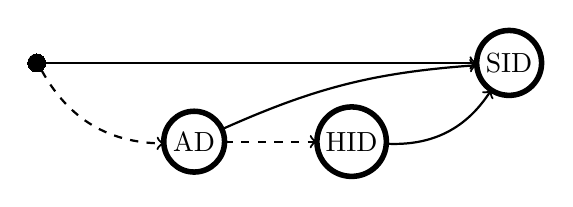
\begin{tikzpicture}
  \entrynode{A}
  \Vertex[x=6,y=0,L=SID]{B}
  \Vertex[x=2,y=-1,L=AD]{C}
  \Vertex[x=4,y=-1,L=HID]{D}
  \tikzstyle{EdgeStyle}=[->]
  \Edge(A)(B)
  \tikzstyle{EdgeStyle}=[dashed, bend right, ->]
  \Edge(A)(C)
  \tikzstyle{EdgeStyle}=[bend left=10, ->]
  \Edge(C)(B)
  \tikzstyle{EdgeStyle}=[dashed, ->]
  \Edge(C)(D)
  \tikzstyle{EdgeStyle}=[bend right, ->]
  \Edge(D)(B)
\end{tikzpicture}
\caption{A typical DAG with two fallbacks. Note that higher edges have higher priority; SID is the primary intent, so the network attempts to route it first. If a router does not know the location of SID, or does not understand services, it uses the first fallback and instead routes the packet to SID's AD. Once in the AD, if a router cannot find SID, the packet is routed to HID, the second fallback, before finally being delivered to the service.}
\label{fig:proxy-service}
\end{figure}


\subsubsection{Intrinsic Security}
All addresses (or, better put, identifiers) in XIA are \emph{intrinsically secure}; exactly what this means varies among principals. For example, a content identifier (CID) is the cryptographic hash of the content itself, enabling anyone receiving the content to verify its integrity. Hosts and services are required to have a public/private key pair; therefore their corresponding identifiers (HIDs and SIDs) are simply the hashes of public keys. A host can sign any communication it generates with its private key and anyone can publicly verify the signature using the host's ID.

\subsection{Anonymity}
We adopt terminology proposed by Pfitzmann and K\"{o}hntopp~\cite{terminology} to precisely describe various meanings of the term {\em anonymity}:
\begin{description}
\item[Anonymity] The state of not being identifiable within a set of subjects, the {\em anonymity set}.
\item[Unlinkability] Two or more items (e.g., subjects, messages, events, actions, etc.) are no more and no less related than they are related to any other item.
\item[Sender Anonymity] A particular message is not linkable to any sender and no message is linkable to a particular sender.
\item[Recipient Anonymity] A particular message cannot be linked to any recipient and no message is linkable to a particular recipient.
\item[Unobservability] The state of messages being indistinguishable from no messages at all.
\end{description}


\section{Approach}
\label{approach}
\subsection{Proxies}
Nico
\subsection{Temporary SIDs}
David
\subsection{Principal-Based Control}
David


\section{Comparison}
\label{comparison}
\subsection{Services vs. Features}
\subsection{Threats vs. ``Meatures''}


\section{Implementation}
\label{implementation}
We implemented a single proxy and a version of the API.
\subsection{Single Proxy DAG Manipulation}
Nico
\subsection{In-Network Services Issues}
Nico
\subsection{OS Integration and API}
David

\section{Conclusion}
\label{conclusion}

\bibliography{FinalWriteup}{}
\bibliographystyle{plain}
\end{document}